\RequirePackage{currfile}
\documentclass[12pt]{beamer}
\usepackage[utf8]{inputenc}
\usepackage[spanish]{babel}
\usepackage{standalone}
\usepackage{color}
\usepackage{siunitx}
\usepackage{hyperref}
%\hypersetup{colorlinks,linkcolor=,urlcolor=blue}
%\hypersetup{colorlinks,urlcolor=blue}
\usepackage{xcolor,soul}
\usepackage{etoolbox}
\usepackage{amsmath}
\usepackage{amsthm}
\usepackage{physics}
\usepackage{multicol}
\usepackage{bookmark}
\usepackage{longtable}
\usepackage{listings}
\lstset{
basicstyle=\ttfamily,
columns=fullflexible,
breaklines=true
}
\usepackage{graphicx}
\usepackage{tikz}
\usetikzlibrary{matrix, backgrounds, decorations,shapes, arrows.meta}
\usepackage[autostyle,spanish=mexican]{csquotes}
\usepackage[os=win]{menukeys}
\usepackage{pifont}
\usepackage{pbox}
\usepackage{caption}
\captionsetup{font=scriptsize,labelfont=scriptsize}
\usepackage{dcolumn}
\newcolumntype{L}{D{.}{.}{2,5}}

\definecolor{ao}{rgb}{0.0, 0.5, 0.0}
\definecolor{bisque}{rgb}{1.0, 0.89, 0.77}
\definecolor{amber}{rgb}{1.0, 0.75, 0.0}
\definecolor{armygreen}{rgb}{0.29, 0.33, 0.13}
\definecolor{alizarin}{rgb}{0.82, 0.1, 0.26}
\definecolor{cadetblue}{rgb}{0.37, 0.62, 0.63}
\definecolor{deepblue}{rgb}{0,0,0.5}
\definecolor{brown}{rgb}{0.59, 0.29, 0.0}
\definecolor{OliveGreen}{rgb}{0,0.25,0}

\definecolor{Code}{rgb}{0,0,0}
\definecolor{Keywords}{rgb}{255,0,0}
\definecolor{Strings}{rgb}{255,0,255}
\definecolor{Comments}{rgb}{0,0,255}
\definecolor{Numbers}{rgb}{255,128,0}


\newcommand*{\TitleParbox}[1]{\parbox[c]{1.75cm}{\raggedright #1}}%

%\usepackage[sfdefault]{roboto}  %% Option 'sfdefault' only if the base font of the document is to be sans serif

\renewcommand{\arraystretch}{1.5}
\renewcommand{\rmdefault}{cmr}% cmr = Computer Modern Roman
\usefonttheme[onlymath]{serif}

\newcommand{\python}{\texttt{python}}
\newcommand{\textoazul}[1]{\textcolor{blue}{#1}}
\newcommand{\azulfuerte}[1]{\textcolor{blue}{\textbf{#1}}}
\newcommand{\funcionazul}[1]{\textcolor{blue}{\textbf{\texttt{#1}}}}

\newcounter{saveenumi}
\newcommand{\seti}{\setcounter{saveenumi}{\value{enumi}}}
\newcommand{\conti}{\setcounter{enumi}{\value{saveenumi}}}

\linespread{1.5}
\beamertemplatenavigationsymbolsempty
\usefonttheme{professionalfonts}
%\usefonttheme{serif}
\DeclareGraphicsExtensions{.pdf,.png,.jpg}
\renewcommand {\arraystretch}{1.25}
\mode<presentation>
{
  \usetheme{Warsaw}
  \setbeamertemplate{headline}{}
  %\useoutertheme{infolines}
  \useoutertheme{default}
  \setbeamercovered{invisible}
  % or whatever (possibly just delete it)
  \setbeamertemplate{section in toc}[sections numbered]
  \setbeamertemplate{subsection in toc}[subsections numbered]
  \setbeamertemplate{subsection in toc}{\leavevmode\leftskip=3.2em\rlap{\hskip-2em\inserttocsectionnumber.\inserttocsubsectionnumber}\inserttocsubsection\par}
  \setbeamercolor{section in toc}{fg=blue}
  \setbeamercolor{subsection in toc}{fg=blue}
  \setbeamercolor{frametitle}{fg=yellow}

  \setbeamertemplate{footline} 
{
  \leavevmode%
  \hbox{%
  \begin{beamercolorbox}[wd=.333333\paperwidth,ht=2.25ex,dp=1ex,center]{author in head/foot}%
    \usebeamerfont{author in head/foot}\insertsection
  \end{beamercolorbox}%
  \begin{beamercolorbox}[wd=.333333\paperwidth,ht=2.25ex,dp=1ex,center]{title in head/foot}%
    \usebeamerfont{title in head/foot}\textcolor{yellow}{\insertsubsection}
  \end{beamercolorbox}%
  \begin{beamercolorbox}[wd=.333333\paperwidth,ht=2.25ex,dp=1ex,right]{date in head/foot}%
    \usebeamerfont{date in head/foot}\insertshortdate{}\hspace*{2em}
    \insertframenumber{} / \inserttotalframenumber\hspace*{2ex} 
  \end{beamercolorbox}}%
  \vskip0pt%
}
}
\makeatother

\makeatletter
\patchcmd{\beamer@sectionintoc}
  {\vfill}
  {\vskip\itemsep}
  {}
  {}
\makeatother

% \makeatletter
% \patchcmd{\hyper@link@}
%   {{\Hy@tempb}{#4}}
%   {{\Hy@tempb}{\ul{#4}}}
%   {}{}
% \makeatother

\DeclareCaptionFont{white}{\color{white}}
\DeclareCaptionFormat{listing}{\colorbox{gray}{\parbox{0.99\textwidth}{#1#2#3}}}
\captionsetup[lstlisting]{format=listing,labelfont=white,textfont=white}
\renewcommand{\lstlistingname}{Código}

\lstdefinestyle{codigopython}{%
  language=Python,                % choose the language of the code
  %basicstyle=\footnotesize\small,       % the size of the fonts that are used for the code
  numbers=left,                   % where to put the line-numbers
  numberstyle=\scriptsize,      % the size of the fonts that are used for the line-numbers
  stepnumber=1,                   % the step between two line-numbers. If it is 1 each line will be numbered
  numbersep=5pt,                  % how far the line-numbers are from the code
  backgroundcolor=\color{white},  % choose the background color. You must add \usepackage{color}
  showspaces=false,               % show spaces adding particular underscores
  showstringspaces=false,         % underline spaces within strings
  showtabs=false,                 % show tabs within strings adding particular underscores
  frame=single,   		% adds a frame around the code
  tabsize=2,  		% sets default tabsize to 2 spaces
  captionpos=t,   		% sets the caption-position to bottom
  breaklines=true,    	% sets automatic line breaking
  breakatwhitespace=false,    % sets if automatic breaks should only happen at whitespace
  escapeinside={\#},  % if you want to add a comment within your code
  stringstyle =\color{OliveGreen},
  texcl = true,
  %otherkeywords={{as}},             % Add keywords here
  keywordstyle = \color{blue},
  commentstyle = \color{black},
  identifierstyle = \color{black},
  % literate=%
  %         {á}{{\'a}}1
  %         {é}{{\'e}}1
  %         {í}{{\'i}}1
  %         {ó}{{\'o}}1
  %         {ú}{{\'u}}1
  %
  %keywordstyle=\ttb\color{deepblue}
  %fancyvrb = true,
literate={0}{{\textcolor{red}{0}}}{1}%
            {1}{{\textcolor{red}{1}}}{1}%
            {2}{{\textcolor{red}{2}}}{1}%
            {3}{{\textcolor{red}{3}}}{1}%
            {4}{{\textcolor{red}{4}}}{1}%
            {5}{{\textcolor{red}{5}}}{1}%
            {6}{{\textcolor{red}{6}}}{1}%
            {7}{{\textcolor{red}{7}}}{1}%
            {8}{{\textcolor{red}{8}}}{1}%
            {9}{{\textcolor{red}{9}}}{1}%
            {.0}{{\textcolor{red}{.0}}}{2}% Following is to ensure that only periods
            {.1}{{\textcolor{red}{.1}}}{2}% followed by a digit are changed.
            {.2}{{\textcolor{red}{.2}}}{2}%
            {.3}{{\textcolor{red}{.3}}}{2}%
            {.4}{{\textcolor{red}{.4}}}{2}%
            {.5}{{\textcolor{red}{.5}}}{2}%
            {.6}{{\textcolor{red}{.6}}}{2}%
            {.7}{{\textcolor{red}{.7}}}{2}%
            {.8}{{\textcolor{red}{.8}}}{2}%
            {.9}{{\textcolor{red}{.9}}}{2}%
            {\ }{{ }}{1}% handle the space
        ,%
        %mathescape=true
        %escapeinside={*@}
        escapeinside={A_}{_B}
}

\usepackage[os=win]{menukeys}
\usepackage{pifont}
\usepackage{caption}
\captionsetup{font=scriptsize,labelfont=scriptsize}
\definecolor{ao}{rgb}{0.0, 0.5, 0.0}
\definecolor{bisque}{rgb}{1.0, 0.89, 0.77}
\definecolor{amber}{rgb}{1.0, 0.75, 0.0}
\definecolor{armygreen}{rgb}{0.29, 0.33, 0.13}
\definecolor{alizarin}{rgb}{0.82, 0.1, 0.26}
\definecolor{cadetblue}{rgb}{0.37, 0.62, 0.63}
%%\RequirePackage[l2tabu, orthodox]{nag}
\RequirePackage{currfile}
\documentclass[12pt]{beamer}
\graphicspath{{Imagenes/}{../Imagenes/}}
\usepackage[utf8]{inputenc}
\usepackage[spanish]{babel}
\usepackage{standalone}
\usepackage{color}
\usepackage[binary-units=true]{siunitx}
\usepackage{hyperref}
\hypersetup{
  colorlinks=true,
  linkcolor=blue,          % color of internal links (change box color with linkbordercolor)
  citecolor=green,        % color of links to bibliography
  filecolor=magenta,      % color of file links
  urlcolor=cyan,           % color of external links
  linkbordercolor={0 0 1}
}
\usepackage{xcolor, soul}
\usepackage{etoolbox}
\usepackage{amsmath}
\usepackage{amsthm}
\usepackage{physics}
\usepackage{multicol}
\usepackage{graphicx}
\usepackage{bookmark}
\usepackage{longtable}
\usepackage{graphicx}
\usepackage{tikz}
\usepackage[siunitx, RPvoltages]{circuitikz}
\usetikzlibrary{mindmap}
\usetikzlibrary{arrows, patterns, shapes, decorations.markings, decorations.pathmorphing}
\usetikzlibrary{matrix,positioning}
\tikzstyle{every picture}+=[remember picture,baseline]
\usepackage[autostyle,spanish=mexican]{csquotes}
\usepackage{pifont}
\usepackage[font=footnotesize,textfont=it]{caption}
\usepackage{tabulary}
\usepackage{booktabs}
\usepackage[outdir=./]{epstopdf}
%\usepackage{epstopdf}
\usepackage{media9}
\usepackage{multimedia}
\usepackage{bigints}
%\usepackage{enumitem}
\usepackage[os=win]{menukeys}
\usepackage{pifont}
\usepackage{pbox}
\usepackage{alltt}
\usepackage{verbatim}
\usepackage{colortbl}
\usepackage{tcolorbox}
\usepackage{fancyvrb}
\usepackage[sfdefault]{roboto}  %% Option 'sfdefault' only if the base font of the document is to be sans serif
%\usepackage[T1]{fontenc}
\setcounter{secnumdepth}{3}
\setcounter{tocdepth}{3}
\DeclareGraphicsExtensions{.pdf,.png,.jpg}
\renewcommand {\arraystretch}{1.5}
\definecolor{ao}{rgb}{0.0, 0.5, 0.0}
\definecolor{aquamarine}{rgb}{0.5, 1.0, 0.83}
\definecolor{kellygreen}{rgb}{0.3, 0.73, 0.09}
\definecolor{bisque}{rgb}{1.0, 0.89, 0.77}
\definecolor{amber}{rgb}{1.0, 0.75, 0.0}
\definecolor{armygreen}{rgb}{0.29, 0.33, 0.13}
\definecolor{alizarin}{rgb}{0.82, 0.1, 0.26}
\definecolor{cadetblue}{rgb}{0.37, 0.62, 0.63}
\newcommand*{\TitleParbox}[1]{\parbox[c]{6cm}{\raggedright #1}}%
\newcommand{\python}{\texttt{python}}
\newcommand{\textoazul}[1]{\textcolor{blue}{#1}}
\newcommand{\azulfuerte}[1]{\textcolor{blue}{\textbf{#1}}}
\newcommand{\funcionazul}[1]{\textcolor{blue}{\textbf{\texttt{#1}}}}
%\normalfont
\usepackage{ccfonts}% http://ctan.org/pkg/{ccfonts}
\usepackage[T1]{fontenc}% http://ctan.or/pkg/fontenc
\renewcommand{\rmdefault}{cmr}% cmr = Computer Modern Roman
\usefonttheme[onlymath]{serif}
\linespread{1.3}
\newcounter{saveenumi}
\newcommand{\seti}{\setcounter{saveenumi}{\value{enumi}}}
\newcommand{\conti}{\setcounter{enumi}{\value{saveenumi}}}
\newcommand{\tikzmark}[1]{\tikz[remember picture] \node[coordinate] (#1) {#1};}

\usepackage{scalerel}[2016-12-29]
\def\stretchint#1{\vcenter{\hbox{\stretchto[440]{\displaystyle\int}{#1}}}}
\def\scaleint#1{\vcenter{\hbox{\scaleto[3ex]{\displaystyle\int}{#1}}}}
\def\bs{\mkern-12mu}

\newtheorem{teo}{}[section]
\usepackage{blkarray}

%reduce el tamaño de letra de la etiqueta equations
\makeatletter
\def\maketag@@@#1{\hbox{\m@th\normalfont\small#1}}
\makeatother

%se usa para la x en itemize
\newcommand{\xmark}{\text{\ding{55}}}

%\AtBeginDocument{\setlength{\tymin}{1em}}


\definecolor{myblue}{rgb}{.8, .8, 1}

\usepackage{empheq}

\newlength\mytemplen
\newsavebox\mytempbox

\makeatletter
\newcommand\mybluebox{%
    \@ifnextchar[%]
       {\@mybluebox}%
       {\@mybluebox[0pt]}}

\def\@mybluebox[#1]{%
    \@ifnextchar[%]
       {\@@mybluebox[#1]}%
       {\@@mybluebox[#1][0pt]}}

\def\@@mybluebox[#1][#2]#3{
    \sbox\mytempbox{#3}%
    \mytemplen\ht\mytempbox
    \advance\mytemplen #1\relax
    \ht\mytempbox\mytemplen
    \mytemplen\dp\mytempbox
    \advance\mytemplen #2\relax
    \dp\mytempbox\mytemplen
    \colorbox{myblue}{\hspace{1em}\usebox{\mytempbox}\hspace{1em}}}

\makeatother



%\usetheme{CambridgeUS}
%%Se usa la plantilla Warsaw modificada con spruce
\mode<presentation>
{
  \usetheme{Berlin}
  \setbeamertemplate{headline}{}
  \useoutertheme{default}
  \usecolortheme{beaver}
  \setbeamercovered{invisible}
}
%\AtBeginSection[]
%{
%\begin{frame}<beamer>{Contenido}
%\normalfont\mdseries
%\tableofcontents[currentsection]
%\end{frame}
%}

\setbeamertemplate{section in toc}[sections numbered]
\setbeamertemplate{subsection in toc}[subsections numbered]
\setbeamertemplate{subsection in toc}{\leavevmode\leftskip=3.2em\rlap{\hskip-2em\inserttocsectionnumber.\inserttocsubsectionnumber}\inserttocsubsection\par}
\setbeamercolor{section in toc}{fg=blue}
\setbeamercolor{subsection in toc}{fg=blue}
\setbeamertemplate{navigation symbols}{}
\setbeamercolor{frametitle}{fg=amber,bg=armygreen}
%\setbeamercolor{frametitle}{fg=blue,bg=ao!90!white}
\setbeamercolor{section in head/foot}{bg=gray!30,fg=red}
%\setbeamercolor{section in head}{bg=green,fg=red}
\setbeamercolor{subsection in head/foot}{bg=gray!30,fg=black}
\setbeamercolor{author in head/foot}{bg=gray!30}
\setbeamercolor{date in head/foot}{fg=blue}

%\mode<presentation>
%{
%  \usetheme{Warsaw}
%  \setbeamertemplate{headline}{}
%  %\useoutertheme{infolines}
%  \useoutertheme{default}
%  \setbeamercovered{invisible}
%  % or whatever (possibly just delete it)
%}

%\usepackage[backend=biber]{biblatex}
%\bibliography{LibrosFC.bib}
%\usepackage{courier}
\usepackage{listingsutf8}
\usepackage{listings}
\usepackage{xcolor}
\usepackage{textcomp}
\usepackage{color}
\definecolor{deepblue}{rgb}{0,0,0.5}
\definecolor{brown}{rgb}{0.59, 0.29, 0.0}
\definecolor{OliveGreen}{rgb}{0,0.25,0}
% \usepackage{minted}

\DeclareCaptionFont{white}{\color{white}}
\DeclareCaptionFormat{listing}{\colorbox{gray}{\parbox{0.98\textwidth}{#1#2#3}}}
\captionsetup[lstlisting]{format=listing,labelfont=white,textfont=white}
\renewcommand{\lstlistingname}{Código}


\definecolor{Code}{rgb}{0,0,0}
\definecolor{Keywords}{rgb}{255,0,0}
\definecolor{Strings}{rgb}{255,0,255}
\definecolor{Comments}{rgb}{0,0,255}
\definecolor{Numbers}{rgb}{255,128,0}

\makeatletter

\newif\iffirstchar\firstchartrue
\newif\ifstartedbyadigit
\newif\ifprecededbyequalsign

\newcommand\processletter
{%
  \ifnum\lst@mode=\lst@Pmode%
    \iffirstchar%
        \global\startedbyadigitfalse%
      \fi
      \global\firstcharfalse%
    \fi
}

\newcommand\processdigit
{%
  \ifnum\lst@mode=\lst@Pmode%
      \iffirstchar%
        \global\startedbyadigittrue%
      \fi
      \global\firstcharfalse%
  \fi
}

\lst@AddToHook{OutputOther}%
{%
  \lst@IfLastOtherOneOf{=}
    {\global\precededbyequalsigntrue}
    {}%
}

\lst@AddToHook{Output}%
{%
  \ifprecededbyequalsign%
      \ifstartedbyadigit%
        \def\lst@thestyle{\color{orange}}%
      \fi
    \fi
  \global\firstchartrue%
  \global\startedbyadigitfalse%
  \global\precededbyequalsignfalse%
}

\lstset{ 
language=Python,                % choose the language of the code
basicstyle=\footnotesize\ttfamily,       % the size of the fonts that are used for the code
numbers=left,                   % where to put the line-numbers
numberstyle=\scriptsize,      % the size of the fonts that are used for the line-numbers
stepnumber=1,                   % the step between two line-numbers. If it is 1 each line will be numbered
numbersep=5pt,                  % how far the line-numbers are from the code
backgroundcolor=\color{white},  % choose the background color. You must add \usepackage{color}
showspaces=false,               % show spaces adding particular underscores
showstringspaces=false,         % underline spaces within strings
showtabs=false,                 % show tabs within strings adding particular underscores
frame=single,   		% adds a frame around the code
tabsize=2,  		% sets default tabsize to 2 spaces
captionpos=t,   		% sets the caption-position to bottom
breaklines=true,    	% sets automatic line breaking
breakatwhitespace=false,    % sets if automatic breaks should only happen at whitespace
escapeinside={\#},  % if you want to add a comment within your code
stringstyle =\color{OliveGreen},
%otherkeywords={{as}},             % Add keywords here
keywordstyle = \color{blue},
commentstyle = \color{black},
identifierstyle = \color{black},
literate=%
         {á}{{\'a}}1
         {é}{{\'e}}1
         {í}{{\'i}}1
         {ó}{{\'o}}1
         {ú}{{\'u}}1
%
%keywordstyle=\ttb\color{deepblue}
%fancyvrb = true,
}

\lstdefinestyle{FormattedNumber}{%
    literate={0}{{\textcolor{red}{0}}}{1}%
             {1}{{\textcolor{red}{1}}}{1}%
             {2}{{\textcolor{red}{2}}}{1}%
             {3}{{\textcolor{red}{3}}}{1}%
             {4}{{\textcolor{red}{4}}}{1}%
             {5}{{\textcolor{red}{5}}}{1}%
             {6}{{\textcolor{red}{6}}}{1}%
             {7}{{\textcolor{red}{7}}}{1}%
             {8}{{\textcolor{red}{8}}}{1}%
             {9}{{\textcolor{red}{9}}}{1}%
             {.0}{{\textcolor{red}{.0}}}{2}% Following is to ensure that only periods
             {.1}{{\textcolor{red}{.1}}}{2}% followed by a digit are changed.
             {.2}{{\textcolor{red}{.2}}}{2}%
             {.3}{{\textcolor{red}{.3}}}{2}%
             {.4}{{\textcolor{red}{.4}}}{2}%
             {.5}{{\textcolor{red}{.5}}}{2}%
             {.6}{{\textcolor{red}{.6}}}{2}%
             {.7}{{\textcolor{red}{.7}}}{2}%
             {.8}{{\textcolor{red}{.8}}}{2}%
             {.9}{{\textcolor{red}{.9}}}{2}%
             {\ }{{ }}{1}% handle the space
         ,%
          %mathescape=true
          escapeinside={__}
          }



%\setbeamercolor{section in foot}{fg=white, bg=BlueViolet}
\makeatletter
\setbeamertemplate{footline}
{
  \leavevmode%
  \hbox{%
  \begin{beamercolorbox}[wd=.333333\paperwidth,ht=2.25ex,dp=1ex,center]{author in head/foot}%
    \usebeamerfont{section in /foot} {\insertsection}
  \end{beamercolorbox}%
  \begin{beamercolorbox}[wd=.333333\paperwidth,ht=2.25ex,dp=1ex,center]{title in head/foot}%
    \usebeamerfont{section in head/foot} {\insertsubsection}
  \end{beamercolorbox}%
  \begin{beamercolorbox}[wd=.333333\paperwidth,ht=2.25ex,dp=1ex,right]{date in head/foot}%
    \usebeamerfont{date in head/foot}\insertshortdate{}\hspace*{2em}
    \insertframenumber{} / \inserttotalframenumber\hspace*{2ex} 
  \end{beamercolorbox}}%
  \vskip0pt%
}
\makeatother

\title{Tema 0 - Introducción a \python}
%\subtitle{Semestre 2018-2}
\author[]{M. en C. Gustavo Contreras Mayén \\ M. en C. Abraham Lima Buendía}
\institute{Facultad de Ciencias - UNAM}
\titlegraphic{
\includegraphics[width=2cm]{escudo-facultad-ciencias}\hspace*{4.75cm}~%
   
\includegraphics[width=2cm]{escudo-unam}
}
\date{\today}
\begin{document}
\maketitle
\section*{Contenido}
\frame[allowframebreaks]{\tableofcontents[currentsection, hideallsubsections]}
\fontsize{14}{14}\selectfont
\spanishdecimal{.}
\section{Usando \python{} con linux}
\frame{\tableofcontents[currentsection, hideothersubsections]}
\subsection{Trabajo en la terminal}
\begin{frame}
\frametitle{La terminal de comandos en linux}
Dentro de un entorno linux, es necesario la operación de comandos, programas, etc. dentro de una terminal.
\\
\bigskip
Que es una ventana en donde debemos de escribir los comandos necesarios para que el sistema operativo ejecute la tarea.
\end{frame}
\begin{frame}
\frametitle{Abrir una terminal en linux}
Con la siguiente combinación de teclas, tendremos una terminal en la pantalla de nuestro equipo:
\\
\bigskip
\bigskip
\begin{center}
\keys{\ctrl + \Alt + t}
\end{center}
\end{frame}
\begin{frame}
\frametitle{La terminal común en linux}
\begin{figure}
	\centering
	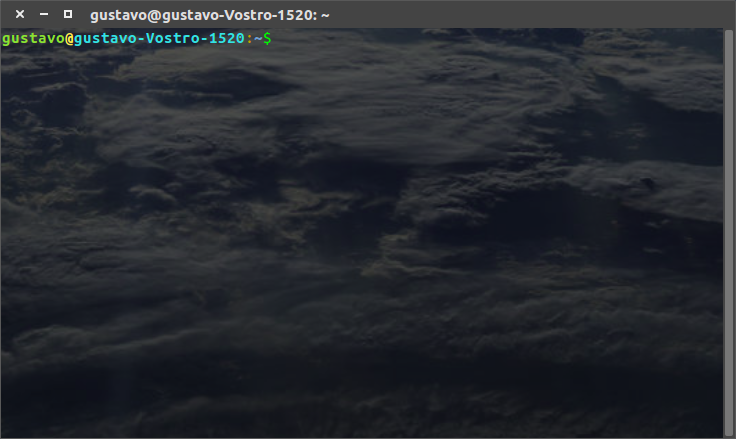
\includegraphics[scale=0.25]{Terminal_01}
	\caption{Pantalla de una terminal en linux.}
\end{figure}
\end{frame}
\begin{frame}
\frametitle{El prompt de la terminal}
En la terminal vemos el llamado \enquote{prompt}, que es el símbolo de dinero  \textasciitilde $\$$
\\
\bigskip
A partir de este momento, linux está en la espera de las instrucciones que ingresemos con el teclado.
\end{frame}
\begin{frame}
\frametitle{Precauciones}
Tengan en cuenta que linux es un sistema operativo diferente, ya que una vez que tecleemos \keys{\return} (la tecla \textbf{Enter}) no se nos pide alguna confirmación, sencillamente se ejecuta la instrucción.
\end{frame}
\begin{frame}
\frametitle{Usar python desde la terminal}
Para usar \python{} desde la terminal, basta con que ingresemos la siguiente instrucción en la terminal:
\begin{center}
\textasciitilde $\$$ \texttt{python} \keys{\return}
\end{center}
\end{frame}
\begin{frame}
\frametitle{Usar python desde la terminal}
\begin{figure}
	\centering
	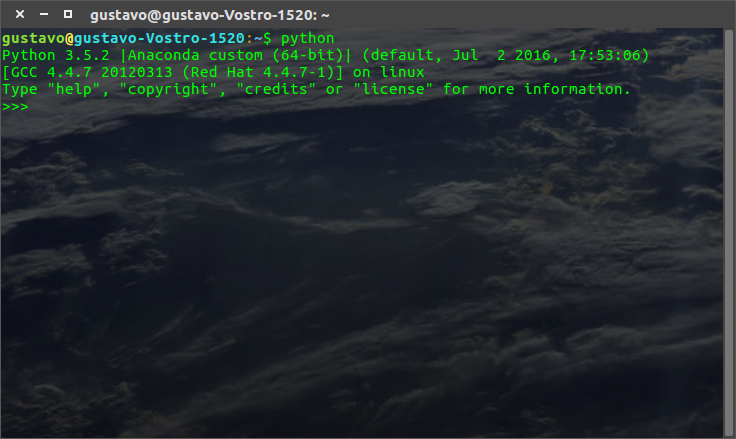
\includegraphics[scale=0.25]{Terminal_02}
	\caption{Vemos cierta información sobre la versión de python instalada en nuestro equipo.}
\end{figure}
\end{frame}
\begin{frame}
\frametitle{El entorno de python en la terminal}
Una vez que ya ingresamos al entorno de \python{} desde la terminal, destacamos el hecho de que el prompt ya cambió: ahora se presenta como $>>>$
\\
\bigskip
Y de nueva cuenta, ahora las instrucciones se deben de escribir en la línea de comandos, pero son instrucciones del lenguaje \python.	
\end{frame}
\begin{frame}
\frametitle{Todo listo para trabajar con \python}
Para ver un saludo en pantalla, escribimos lo siguiente:
\begin{center}
$>>>$ \texttt{print("Hola mundo!")} \keys{\return}
\end{center}
\end{frame}
\begin{frame}
\frametitle{Todo listo para trabajar con \python}
\begin{figure}
	\centering
	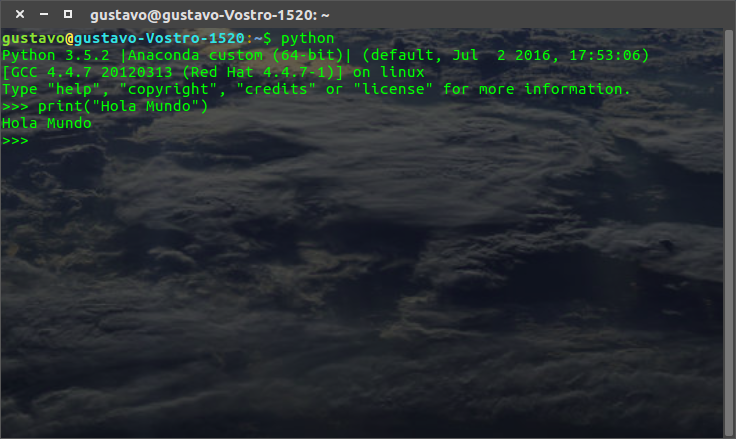
\includegraphics[scale=0.25]{Terminal_03}
	\caption{Obtenemos la respuesta en la siguente línea de la terminal de \python.}
\end{figure}
\end{frame}
\begin{frame}
\frametitle{Salir del entorno de \python{} en la terminal}
Par salir del entorno de python en la terminal de linux, basta con escribir:
\begin{center}
$>>>$ \texttt{exit()} \keys{\return}
\end{center}
\end{frame}
\begin{frame}
\frametitle{Salir del entorno de \python{} en la terminal}
\begin{figure}
	\centering
	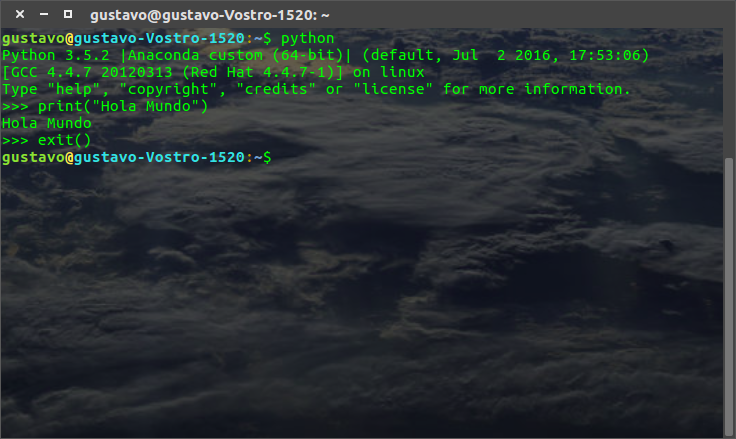
\includegraphics[scale=0.25]{Terminal_04}
	\caption{Regresamos al entorno de linux, revisa el prompt de la terminal.}
\end{figure}
\end{frame}
{
\setbeamercolor{frametitle}{fg=bisque,bg=ao!90!white}
\begin{frame}
\frametitle{Entorno más agradable de trabajo}
El entorno de trabajo para \python{} en la terminal se vuelve en ocasiones muy tedioso, no hay manera de mejorar más allá de la tipografía y fondo de la terminal.
\\
\bigskip
Pero podemos aprovechar al máximo otra herramienta para el curso: \textoazul{\texttt{qtConsole}}, que está integrada en Anaconda\footnote{Revisa la guía de instalación de la suite Anaconda}.
\end{frame}
\begin{frame}
\frametitle{Usaremos ahora qtConsole}
Para trabajar con \textoazul{qtConsole}, con la terminal llamamos a la suite anaconda, por lo que escribrimos:
\begin{center}
\textasciitilde $\$$ \texttt{anaconda-navigator} \keys{\return}
\end{center}
\end{frame}
\begin{frame}
\frametitle{Veremos ahora la pantalla de Anaconda}
\begin{figure}
	\centering
	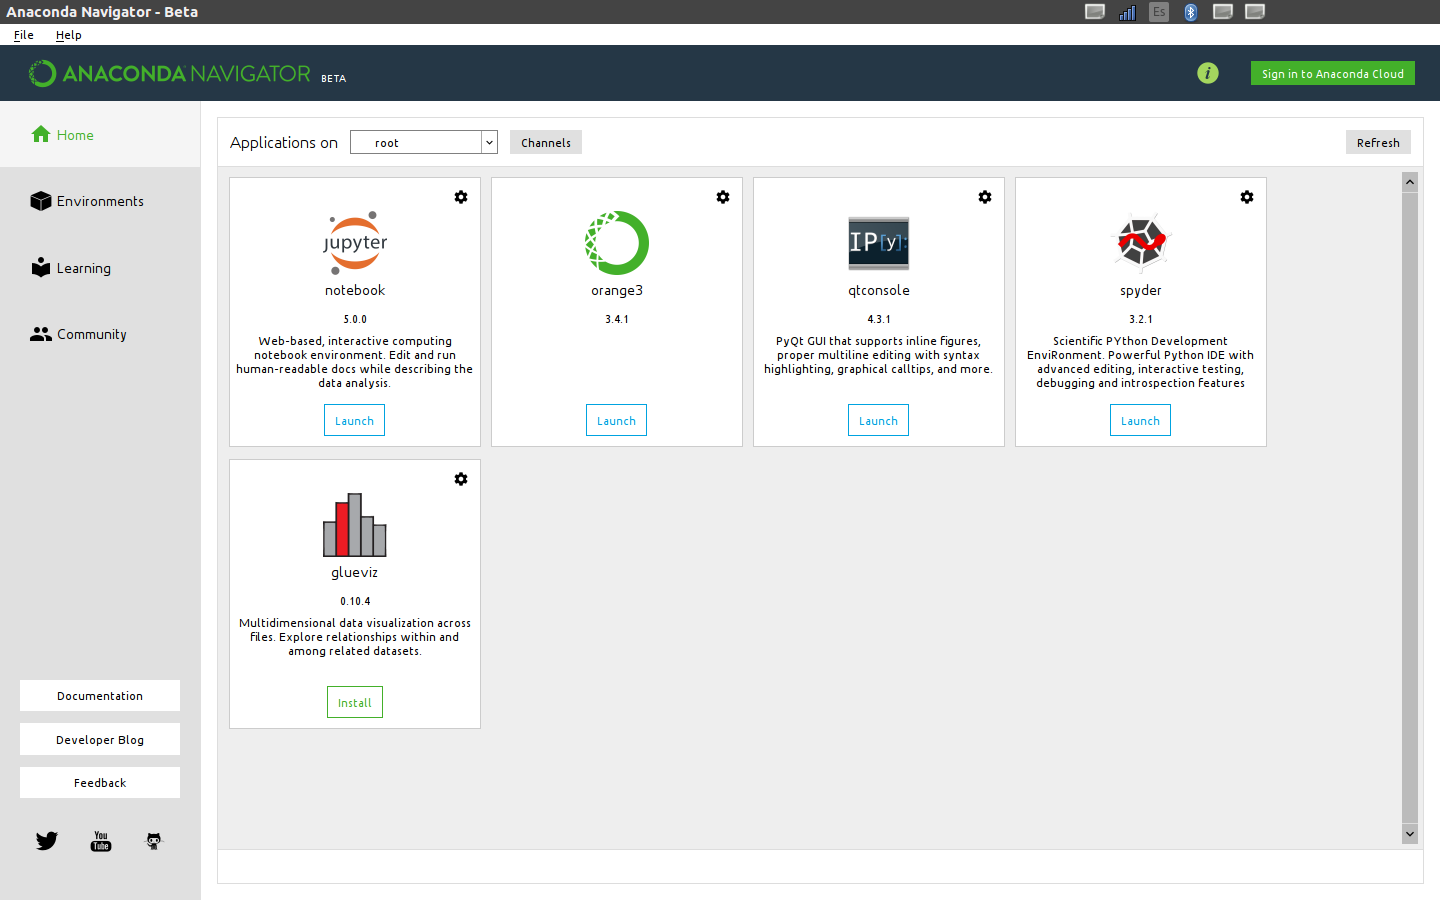
\includegraphics[scale=0.2]{anaconda_01.png}
	%\caption{La suite Anaconda}
\end{figure}
\end{frame}
\begin{frame}
\frametitle{Elegimos qtConsole}
\begin{figure}
	\centering
	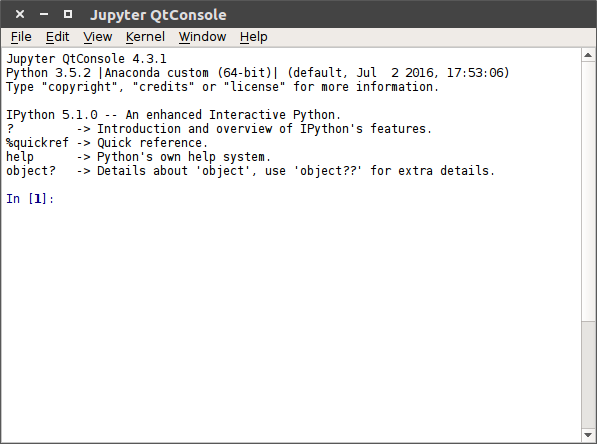
\includegraphics[scale=0.35]{qtConsole_01.png}
	\caption{La ventana de trabajo de qtConsole}
\end{figure}
\end{frame}
\begin{frame}
\frametitle{La ventana de qtConsole}
\begin{figure}
	\centering
	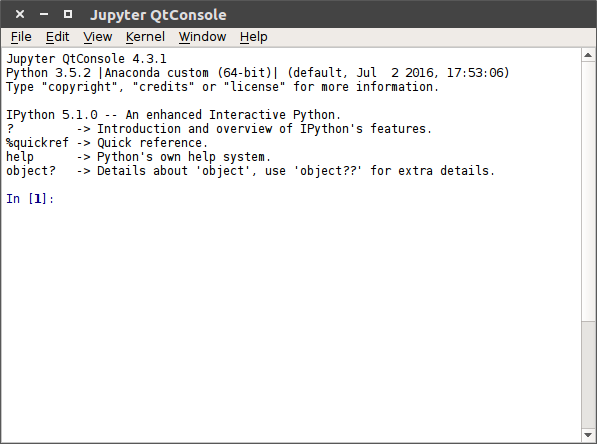
\includegraphics[scale=0.35]{qtConsole_01.png}
	\caption{La ventana de trabajo de qtConsole}
\end{figure}
\end{frame}
\section{Anaconda y python}
\frame{\tableofcontents[currentsection, hideothersubsections]}
\subsection{Usando Anaconda}
\begin{frame}
\frametitle{Personalización de qtConsole}
\begin{figure}
	\centering
	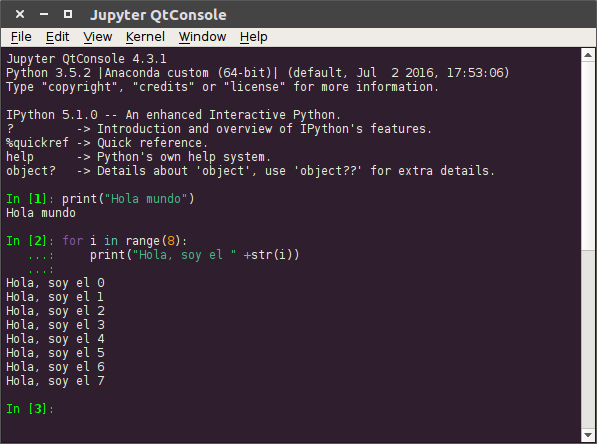
\includegraphics[scale=0.35]{qtConsole_02}
	\caption{Podemos pesonalizar la ventana de trabajo}
\end{figure}
\end{frame}
\begin{frame}
\frametitle{Combinación de estilos}
\begin{figure}
	\centering
	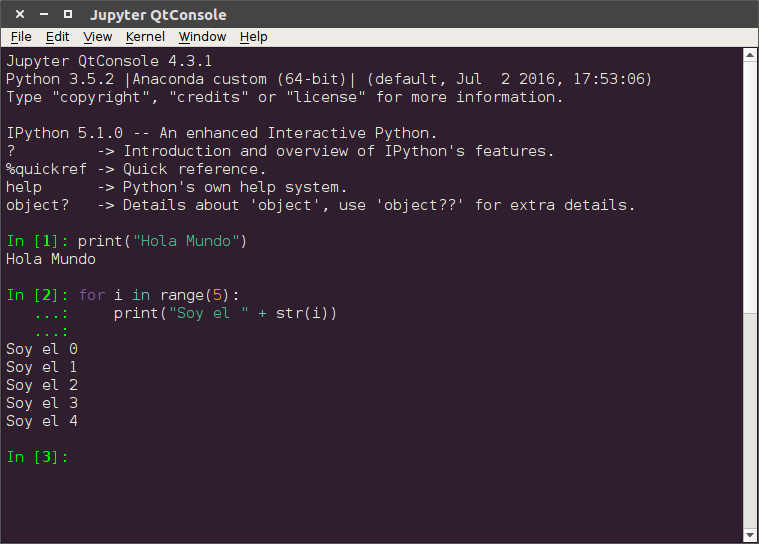
\includegraphics[scale=0.3]{qtConsole_03}
	\caption{Cambio en la tipografía y tamaño de letra en qtConsole}
\end{figure}
\end{frame}
\section{python como una calculadora}
\frame{\tableofcontents[currentsection, hideothersubsections]}
\subsection{Operadores aritméticos}
\begin{frame}
\frametitle{\python{} como calculadora}
Una vez abierta la sesión en \python, podemos aprovechar al máximo este lenguaje: contamos con una calculadora a la mano, sólo hay que ir escribiendo las operaciones en la línea de comandos.
\end{frame}
\setbeamercolor{block title}{bg=red!50,fg=black}
\begin{frame}[fragile]
\frametitle{Algunas operaciones}
\begin{block}{Podemos hacer una suma}
\verb|>>>3 + 200| \\
\pause
\verb|203|
\end{block}
\end{frame}
\begin{frame}[fragile]
\begin{block}{Divisón entre enteros}
\verb|>>>30 / 1234| \\
\pause
\verb| 0.024311183144246355|
\end{block}
\end{frame}
\begin{frame}[fragile]
\begin{block}{Una división entre reales}
\verb|>>>3.0 / 4.0| \\
\pause
\verb| 0.75|
\end{block}
\end{frame}
\begin{frame}[fragile]
\begin{block}{Una división entera}
Devuelve el cociente sin decimales \\
\verb|>>>30 // 4| \\
\pause
\verb| 7|
\end{block}
\end{frame}
\begin{frame}[fragile]
\begin{block}{Una división entera}
Otro ejemplo de un cociente sin decimales \\
\verb|>>>4 // 3| \\
\pause
\verb| 1|
\end{block}
\end{frame}
\begin{frame}[fragile]
\frametitle{Combinación de operadores artiméticos}
\begin{block}{Combinando operadores}
\verb|>>>5.0 / 10 * 2 + 5| \\
\pause
\verb| 6.0|
\end{block}
\pause
\textbf{¿por qué obtenemos este resultado??}
\end{frame}
\begin{frame}[fragile]
El resultado cambia cuando agrupamos con paréntesis
\begin{block}{}
\verb|>>>5.0 / (10 * 2 + 5)| \\
\pause
\verb| 0.2|
\end{block}
\pause
Como podemos ver, el uso de paréntesis en las expresiones tiene una  particular importancia sobre la manera en que se evalúan las expresiones.
\end{frame}
\begin{frame}[fragile]
\begin{block}{Potenciación de un número}
Podemos elevar a una potencia en particular, cualquier número
\verb|>>>2 ** 3 ** 2| \\
\pause
\verb| 512|
\end{block}
\pause
\textbf{¿de qué manera se evaluó esta expresión?}
\end{frame}
\begin{frame}[fragile]
\frametitle{Orden en que se evaluán las potencias}
Vemos que elevar a una potencia, la manera en que se ejecuta la expresión se realiza en un sentido en particular: de derecha a izquierda.
\begin{block}{Potenciación de un número}
Podemos elevar a una potencia en particular, cualquier número
\verb|>>>(2 ** 3) ** 2| \\
\pause
\verb| 64|
\end{block}
\pause
El uso de paréntesis nos indica que la expresión contenida dentro de ellos, es la que se evalúa primero, posteriormente se sigue la regla de precedencia de operadores.
\end{frame}
\begin{frame}[fragile]
\begin{block}{Operador módulo}
El operador módulo $\%$ nos devuelve el residuo del cociente.\\
\verb|>>>17 // 3| \\
\pause
\verb| 2|
\end{block}
\end{frame}
\subsection{Tabla de operadores}
\begin{frame}
\frametitle{Tabla de lo operadores aritméticos}
\begin{table}
\fontsize{12}{12}\selectfont
\begin{tabular}{|c | l | c | c|}
\hline
Operador & Operación & Ejemplo & Resultado \\ \hline
$**$ & Potencia & $2**3$ & $8$ \\ \hline
$*$ & Multiplicación & $7*3$ & $21$ \\ \hline
$/$ & División & $10.5/2$ & $5.25$ \\ \hline
$ //$ & Div. entera & $10.5//2 $ & $5.0$ \\ \hline
$+$ & Suma & $3+4$ & $7$ \\ \hline
$-$ & Resta & $6-8$ & $-2$ \\ \hline
$\%$ & Módulo & $15\%6$ & $3$ \\ \hline
\end{tabular}
\end{table}
\end{frame}
\begin{frame}
\frametitle{Precedencia de los operadores aritméticos}
\setbeamercolor{item projected}{bg=blue!70!black,fg=yellow}
\setbeamertemplate{enumerate items}[circle]
\begin{enumerate}[<+->]
\item Las expresiones contenidas dentro de pares de paréntesis son evaluadas primero. En el caso de expresiones con paréntesis anidados, los operadores en el par de paréntesis más interno son aplicados primero.
\item Las operaciones de exponentes son aplicadas después. Si una expresión contiene muchas operaciones de exponentes, los operadores son aplicados de derecha a izquierda.
\end{enumerate}
\end{frame}
\begin{frame}
\frametitle{Precedencia de los operadores aritméticos}
\setbeamercolor{item projected}{bg=blue!70!black,fg=yellow}
\setbeamertemplate{enumerate items}[circle]
\begin{enumerate}[<+->]
\setcounter{enumi}{2}
\item La multiplicación, división y módulo son las siguientes en ser aplicadas. Si una expresión contiene muchas multiplicaciones, divisiones u operaciones de módulo, los operadores se aplican de izquierda a derecha.
\item Suma y resta son las operaciones que se aplican por último. Si una expresión contiene muchas operaciones de suma y resta, los operadores son aplicados de izquierda a derecha. La suma y resta tienen el mismo nivel de precedencia.
\end{enumerate}
\end{frame}
\section{Operadores relaciones en python}
\frame{\tableofcontents[currentsection, hideothersubsections]}
\subsection{Operadores relacionales}
\begin{frame}
\frametitle{Operadores relacionales}
Cuando se comparan dos (o más expresiones) mediante un operador, el tipo de dato que se devuelve es lógico: \textoazul{\textbf{True}} o \textcolor{red}{\textbf{False}}, que también tienen una representación de tipo numérico:
\begin{itemize}
\item \textoazul{\textbf{True}} = $1$
\item \textcolor{red}{\textbf{False}} = $0$
\end{itemize}
\end{frame}
\begin{frame}[fragile]
\frametitle{Operaciones aritméticas y relacionales}
Podemos extender el manejo con \python, al combinar las operaciones aritméticas y relaciones, nótese que siempre tendremos un valor booleano que se devuelve.
\begin{block}{}
\verb|>>> 1 + 2 > 7 - 3| \\
\pause
\verb| False|
\end{block}
\end{frame}
\begin{frame}[fragile]
\begin{block}{}
\verb|>>> 1 < 2 < 3| \\
\pause
\verb| True|
\end{block}
\end{frame}
\begin{frame}[fragile]
\frametitle{El operador de comparación de igualdad}
El doble signo igual ($==$) es el operador de igualdad, a diferencia del operador $=$ que es el operador de asignación.
\begin{block}{}
\verb|>>> 1 > 2 == 2 < 3| \\
\pause
\verb| False|
\end{block}
\end{frame}
\begin{frame}[fragile]
\begin{block}{}
\verb|>>> 3 > 4 < 5| \\
\pause
\verb| False|
\end{block}
\pause
\begin{block}{}
\verb|>>> 1.0 / 3 < 0.3333| \\
\pause
\verb| False|
\end{block}
\pause
\begin{block}{}
\verb|>>> 5.0 / 3 >= 11 /7.0| \\
\pause
\verb| True|
\end{block}
Las expresiones se pueden complicar cada vez más, por lo que hay que mantener atención al momento de escribirlas.
\end{frame}
\begin{frame}
\frametitle{Tabla de operadores relacionales}
\begin{table}
\fontsize{12}{12}\selectfont
\begin{tabular}{| c | l | c | c |}
\hline
Operador & Operación & Ejemplo & Resultado\\ \hline
$==$ & Igual a & $4==5$ & \textcolor{red}{\texttt{False}} \\ \hline
$!=$ & Diferente & $2!=3$ & \textoazul{\texttt{True}} \\ \hline
$<$ & Menor que & $ 10<4$  & \textcolor{red}{\texttt{False}} \\ \hline
$>$ & Mayor que & $5>-4$ & \textoazul{\texttt{True}} \\ \hline
$<=$ & Menor o igual & $7<=7$ & \textoazul{\texttt{True}} \\ \hline
$>=$ & Mayor o igual & $3.5 >= 10$ & \textcolor{red}{\texttt{False}} \\ \hline
\end{tabular}
\end{table}
\end{frame}
\section{Operadores booleanos en python}
\frame{\tableofcontents[currentsection, hideothersubsections]}
\subsection{Operadores booleanos}
\begin{frame}
\frametitle{Operadores booleanos}
En el caso del operador boleano \texttt{and} y el operador \texttt{or} evalúan una expresión compuesta por dos (o más términos).
\\
\bigskip
Si ambas expresiones tienen el valor \textoazul{True}, el valor que devuelve la evaluación de la expresión que involucra a las dos primeras, es \textoazul{True}.
\end{frame}
\begin{frame}
Como se verá en la tabla de verdad, se necesita una condición particular para que el valor que devuelva la comparación, sea \textcolor{red}{\texttt{False}}.
\begin{table}
\fontsize{12}{12}\selectfont
\begin{tabular}{| c | l | c | c |}
\hline
Operador & Operación & Ejemplo & Resultado \\ \hline
\texttt{and} & Conjunción & \textcolor{red}{False} and \textoazul{True} & \textcolor{red}{False} \\ \hline
\texttt{or} & Disyunción & \textcolor{red}{False} or \textoazul{True}  &
\textoazul{True} \\ \hline
\texttt{not} & Negación & \texttt{not} \textoazul{True} & \textcolor{red}{False} \\ \hline
\end{tabular}
\end{table}
\end{frame}
\begin{frame}
\frametitle{Tabla de verdad de los operadores booleanos}
\begin{table}
\begin{tabular}{| c | c | c | c | c |}
\hline
A & B & A \texttt{and} B & A \texttt{or} B & \texttt{not} A\\ \hline
\textoazul{True} & \textoazul{True} & \textoazul{True} & \textoazul{True} & \textcolor{red}{False}\\ \hline
\textoazul{True} & \textcolor{red}{False} & \textcolor{red}{False} & \textoazul{True} & \textcolor{red}{False} \\ \hline
\textcolor{red}{False} & \textoazul{True} & \textcolor{red}{False} & \textoazul{True} & \textoazul{True}\\ \hline
\textcolor{red}{False} & \textcolor{red}{False} & \textcolor{red}{False} & \textcolor{red}{False} & \textoazul{True} \\ \hline
\end{tabular}
\end{table}
\end{frame}
\section{Las variables en \python}
\frame{\tableofcontents[currentsection, hideothersubsections]}
\subsection{Tipos de variables}
\begin{frame}
\frametitle{Tipos de variables}
Las variables en \python{} sólo son ubicaciones de memoria reservadas para almacenar valores.
\\
\bigskip
Esto significa que cuando se crea una variable, se reserva un poco de espacio disponible en la memoria.
\end{frame}
\begin{frame}
Basándose en el tipo de datos de una variable, el intérprete asigna memoria y decide qué se puede almacenar en la memoria reservada.
\\
\bigskip
Por lo tanto, al asignar diferentes tipos de datos a las variables, se pueden almacenar \textbf{enteros}, \textbf{decimales} o \textbf{caracteres (cadenas)} en estas variables.
\end{frame}
\begin{frame}
\frametitle{Asignando valores a variables}
Las variables de \python{} no necesitan una declaración explícita para reservar espacio de memoria.
\\
\bigskip
La declaración ocurre automáticamente cuando se asigna un valor a una variable. \emph{El signo igual (=) se utiliza para asignar valores a las variables}.
\end{frame}
\begin{frame}
El término a la izquierda del operador $=$ es el \emph{nombre de la variable} y el término a la derecha del operador $=$ es el \emph{valor almacenado} en la variable.
\end{frame}
\begin{frame}[fragile]
\frametitle{Ejemplos}
Los comentarios en \python{} se indican con el símbolo $\#$, el texto no se interpreta como una instrucción.
\begin{exampleblock}{}
\fontsize{10}{10}\selectfont
\begin{verbatim}
>>>contador = 100				# Asignacion de tipo entero
>>>distancia = 1000.0			# De punto flotante
>>>nombre = "Chucho"			# Una cadena de caracteres

>>>print(contador)
>>>print(distancia)
>>>print(nombre)
\end{verbatim}
\end{exampleblock}
\end{frame}
\begin{frame}[fragile]
\frametitle{Resultado}
\begin{verbatim}
100
1000.0
Chucho
\end{verbatim}
\end{frame}
\begin{frame}[fragile]
\frametitle{Asignación múltiple de valores}
En \python podemos asignar un valor único a varias variables simultáneamente.
\\
\bigskip
\begin{minipage}{0.37\textwidth}
\begin{verbatim}
>>> A = b = c = 1
>>> print(A)
>>> print(b}
>>> print(c)
\end{verbatim}
\pause
\begin{verbatim}
1
1
1
\end{verbatim}
\end{minipage}
\hspace{1cm}
\pause
\begin{minipage}{0.47\textwidth}
En el ejemplo, se crea un objeto entero con el valor $1$, y las tres variables se asignan a la misma ubicación de memoria.
\end{minipage}
\end{frame}
\begin{frame}[fragile]
\frametitle{Asignación múltiple a varias variables}
También puede asignar varios objetos a varias variables.
\\
\bigskip
\begin{verbatim}
>>> A, b, c = 1, 2, "Alicia"
>>> print (A)
>>> print (b)
>>> print (c)
\end{verbatim}
\pause
\begin{minipage}{0.3\textwidth}
\begin{verbatim}
1
2
Alicia
\end{verbatim}
\end{minipage}
\pause
\hspace{1.5cm}
\begin{minipage}{0.55\textwidth}
\fontsize{12}{12}\selectfont
Aquí, dos objetos enteros con valores $1$ y $2$ se asignan a las variables $A$ y $b$ respectivamente, y un objeto de cadena con el valor \textbf{Alicia} se asigna a la variable $c$.
\end{minipage}
\end{frame}
\section{Tipos de Datos Estándar}
\frame[allowframebreaks]{\tableofcontents[currentsection, hideothersubsections]}
\subsection{Los tipos de datos en \python}
\begin{frame}
Los datos almacenados en la memoria pueden ser de varios tipos. Por ejemplo, la edad de una persona se almacena como un valor numérico y su dirección se almacena como caracteres alfanuméricos.
\\
\bigskip
En \python se cuenta con varios tipos de datos estándar que se utilizan para definir las operaciones posibles entre ellos y el método de almacenamiento para cada uno de ellos.
\end{frame}
\begin{frame}
\frametitle{Tipos de datos}
Los tipos de datos que se utilizan en \python son cinco:
\setbeamercolor{item projected}{bg=blue!70!black,fg=yellow}
\setbeamertemplate{enumerate items}[circle]
\begin{enumerate}[<+->]
\item Números.
\item Cadena.
\item Lista.
\item Tupla.
\item Diccionario.
\end{enumerate}
\end{frame}
\begin{frame}
\frametitle{Números}
Los tipos de datos numéricos almacenan valores numéricos.
\\
\bigskip
Los objetos numéricos se crean cuando se les asigna un valor.
\end{frame}
\begin{frame}[fragile]
\frametitle{Declaración en variables}
\begin{verbatim}
>>> Var1 = Var2 = 10
>>> print (Var1)
>>> print (Var2)
\end{verbatim}
\pause
\begin{verbatim}
10
10
\end{verbatim}
\end{frame}
\begin{frame}
\frametitle{Eliminar variables en \python}
También se puede eliminar la referencia a un objeto numérico utilizando la sentencia \texttt{del}
\\
\bigskip
La sintaxis de la sentencia \texttt{del} es:
\\
\bigskip
\texttt{del var1 [, var2 [, var3 [...., varN]]]]}
\end{frame}
\begin{frame}[fragile]
Se puede eliminar un solo objeto o varios objetos utilizando la sentencia \texttt{del}
\\
\bigskip
Por ejemplo:
\begin{verbatim}
del var

del variable1, variable2
\end{verbatim}
\end{frame}
\subsection{Tipos de datos numéricos}
\begin{frame}
\frametitle{Tipos de datos numéricos}
En python se soportan tres tipos numéricos diferentes:
\setbeamercolor{item projected}{bg=blue!70!black,fg=yellow}
\setbeamertemplate{enumerate items}[circle]
\begin{enumerate}[<+->]
\item Int (enteros con signo)
\item Flotante (valores reales de punto flotante)
\item Complejos (números complejos)
\end{enumerate}
\end{frame}
\begin{frame}
\frametitle{Números enteros}
Los números enteros son aquellos que no tienen decimales, tanto positivos como negativos (además del cero). En \python{} se representan mediante el tipo \texttt{int} (de integer, entero).
\\
\bigskip
Todos los números enteros en \python 3 se representan como enteros largos.
\end{frame}
\begin{frame}
\frametitle{Números reales o flotantes}
Los números reales son los que tienen decimales. En \python{} se expresan mediante el tipo \texttt{float}.
\\
\bigskip
En \python{} se implementa su tipo float utilizando 64 bits, en concreto se sigue el estándar IEEE 754\footnote{En el Tema 1, ampliaremos esta información}: 1 bit para el signo, 11 para el exponente, y 52 para la mantisa.
\end{frame}
\begin{frame}
\frametitle{Números complejos}
Un número complejo consiste en un par ordenado de números reales de coma flotante denotados por
\[ x + y \: j\]
donde $x$ e $y$ son números reales, $y \: j$ es la unidad imaginaria.
\end{frame}
\begin{frame}
\frametitle{Ejemplos de tipos de datos numéricos}
\begin{table}
\begin{tabular}{| c | c | c |}
\hline
\texttt{int} & \texttt{float} & \texttt{complex} \\ \hline
$10$ & $0.0$ & $3.14 \: j$ \\ \hline
$100$ & $15.20$ & $45.j$ \\ \hline
$100$ & $-15.20$ & $23.15+7.5j$ \\ \hline
$080$ & $32.3+e18$ & $0.876j$ \\ \hline
$-0490$ & $-90.$ & $-0.645+0j$ \\ \hline
$-0x260$ & $-32.54e100$ & $3e+26j$ \\ \hline
$0x69$ & $70.2-E12$ & $4.53e-7j$ \\ \hline
\end{tabular}
\end{table}    
\end{frame}
\subsection{Cadenas}
\begin{frame}
\frametitle{Cadenas en python}
Las cadenas en \python{} se identifican como un conjunto contiguo de caracteres representados en las comillas.
\\
\bigskip
Con \python{} se permite cualquier par de 'comillas simples' o comillas \enquote{dobles}.
\end{frame}
\begin{frame}
\frametitle{Operación con cadenas}
Los subconjuntos de cadenas pueden ser tomados usando el operador de corte $[]$ y $[:]$ con los índices comenzando en $0$ al inicio de la cadena hasta llegar a $-1$ al final de la misma.
\pause
El signo más $+$ es el operador de concatenación de cadenas y el asterisco $*$ es el operador de repetición.
\end{frame}
\begin{frame}[fragile]
\frametitle{Ejemplos}
\begin{verbatim}
>>> cadena = 'Hola Mundo!'

>>> print (cadena)
>>> print (cadena[0])
>>> print (cadena[2:5])     
>>> print (cadena[2:])
>>> print (cadena * 2)
>>> print (cadena + "PUMAS")
\end{verbatim}
\end{frame}
\begin{frame}[fragile]
\frametitle{Resultados}
\begin{verbatim}
>>> print (cadena[0])
\end{verbatim}
\pause
Presenta el primer caracter de la cadena
\begin{verbatim}
H
\end{verbatim}
\pause
\begin{verbatim}
>>> print (cadena[2:5])
\end{verbatim}
\pause
Presenta los caracteres de la 3a a la 5a posicion
\begin{verbatim}
la
\end{verbatim}
\end{frame}
\begin{frame}[fragile]
\frametitle{Resultados}
\begin{verbatim}
>>> print (cadena[2:])
\end{verbatim}
\pause
Presenta la cadena que inicia a partir del 3er caracter
\begin{verbatim}
la Mundo!
\end{verbatim}
\pause
\begin{verbatim}
>>> print (cadena * 2)
\end{verbatim}
\pause
Presenta dos veces la cadena
\begin{verbatim}
Hola Mundo!Hola Mundo!
\end{verbatim}
\end{frame}
\begin{frame}[fragile]
\frametitle{Resultados}
\begin{verbatim}
>>> print (cadena + "PUMAS")
\end{verbatim}
\pause
Presenta la cadena y concatena la segunda cadena
\begin{verbatim}
Hola Mundo!PUMAS
\end{verbatim}
\end{frame}
\subsection{Listas}
\begin{frame}
\frametitle{Lista in \python}
Las listas es el tipo de dato más versátil de los tipos de datos compuestos de \python.
\\
\bigskip
Una lista contiene elementos separados por comas y entre corchetes $[ ]$.
\end{frame}
\begin{frame}
En cierta medida, las listas son similares a los arreglos (arrays) en el lenguaje C.
\\
\bigskip
Una de las diferencias entre ellos es que todos los elementos pertenecientes a una lista pueden ser de tipo de datos diferente.
\end{frame}
\begin{frame}
Los valores almacenados en una lista se pueden acceder utilizando el operador de división $[ \: ]$ y $[:]$ con índices que empiezan en $0$ al principio de la lista y opera hasta el final con $-1$.
\\
\bigskip
El signo más $+$ es el operador de concatenación de lista y el asterisco $*$ es el operador de repetición.
\end{frame}
\begin{frame}[fragile]
\frametitle{Ejemplos con listas}
\fontsize{12}{12}\selectfont
\begin{verbatim}
milista = [ 'abcd', 786 , 2.23, 'salmon', 70.2 ]

listabreve = [123, 'pizza']
\end{verbatim}
\end{frame}
\begin{frame}[fragile]
\frametitle{Operaciones con las listas}
\begin{verbatim}
>>> print (milista)
\end{verbatim}
\pause
\begin{verbatim}
['abcd', 786, 2.23, 'salmon', 70.2]
\end{verbatim}
\pause
\begin{verbatim}
>>> print (milista[0])
\end{verbatim}
\pause
\begin{verbatim}
abcd
\end{verbatim}
\pause
\begin{verbatim}
>>> print (milista[1:3])
\end{verbatim}
\pause
\begin{verbatim}
[786, 2.23]
\end{verbatim}
\end{frame}
\begin{frame}[fragile]
\frametitle{Operaciones con las listas 2}
\begin{verbatim}
>>> print (milista[2:])
\end{verbatim}
\pause
\begin{verbatim}
[2.23, 'salmon', 70.2]
\end{verbatim}
\pause
\begin{verbatim}
>>> print (listabreve * 2)
\end{verbatim}
\pause
\begin{verbatim}
[123, 'pizza', 123, 'pizza']
\end{verbatim}
\pause
\begin{verbatim}
>>> print (milista + listabreve)
\end{verbatim}
\pause
\begin{verbatim}
['abcd', 786, 2.23, 'salmon', 70.2, 123, 'pizza']
\end{verbatim}
\end{frame}
\subsection{Tuplas}
\begin{frame}
\frametitle{Tuplas en \python}
Una tupla es otro tipo de datos de secuencia que es similar a la lista.
\\
\bigskip
Una tupla consiste en un número de valores separados por comas. Sin embargo, a diferencia de las listas, las tuplas se incluyen entre paréntesis.
\end{frame}
\begin{frame}
\frametitle{Diferencias entre listas y tuplas}
Las principales diferencias entre las listas y las tuplas son:
\setbeamercolor{item projected}{bg=blue!70!black,fg=yellow}
\setbeamertemplate{enumerate items}[circle]
\begin{enumerate}[<+->]
\item Las listas están entre corchetes $[\;]$ y sus elementos y tamaño pueden cambiarse.
\item Las tuplas están entre paréntesis $(\;)$ y \emph{no se pueden actualizar}.
\end{enumerate}
\pause
Las tuplas pueden ser consideradas como listas de sólo lectura.
\end{frame}
\begin{frame}[fragile]
\frametitle{Ejemplos con tuplas}
\begin{verbatim}
mitupla = ( 'abcd', 786 , 2.23, 'arena', 70.2  )
tuplabreve = (123, 'playa')
\end{verbatim}
\pause
\begin{verbatim}
>>> print (mitupla)
\end{verbatim}
\pause
\begin{verbatim}
('abcd', 786, 2.23, 'arena', 70.2)
\end{verbatim}
\pause
\begin{verbatim}
>>> print (mitupla[0])
\end{verbatim}
\pause
\begin{verbatim}
abcd
\end{verbatim}
\end{frame}
\begin{frame}[fragile]
\frametitle{Ejemplos con tuplas 2}
\begin{verbatim}
>>> print (mitupla[1:3])
\end{verbatim}
\pause
\begin{verbatim}
(2.23, 'arena', 70.2)
\end{verbatim}
\pause
\begin{verbatim}
>>> print (tuplabreve * 2)  
\end{verbatim}
\pause
\begin{verbatim}
(123, 'playa', 123, 'playa')
\end{verbatim}
\pause
\begin{verbatim}
>>> print (mitupla + tuplabreve)
\end{verbatim}
\pause
\begin{verbatim}
('abcd', 786, 2.23, 'arena', 70.2, 123, 'playa')
\end{verbatim}
\end{frame}
\begin{frame}[fragile]
\frametitle{Errores con el manejo de tuplas}
El siguiente código es inválido con la tupla, porque intentamos actualizar una tupla, ya que la acción de incluir un elemento en la tupla no está permitida.
\begin{verbatim}
>>> mitupla = ( 'abcd', 786 , 2.23, 'edificio', 70.2  )
>>> mitupla[2] = 1000
\end{verbatim}
\fontsize{8}{8}\selectfont
\begin{verbatim}
-----------------------------

 TypeError           Traceback (most recent call last)

<ipython-input-19-a99f473d7b8f> in <module>()
       1 mitupla = ( 'abcd', 786 , 2.23, 'edificio', 70.2  )
       2 mitupla[2] = 1000

 TypeError: 'tuple' object does not support item assignment
\end{verbatim}
\end{frame}
\begin{frame}[fragile]
\frametitle{Agregar elementos a la lista}
Pero en la lista podemos agregar nuevos elementos que se colocan al  final de la misma:
\begin{verbatim}
>>> print(milista)
[ 'abcd', 786 , 2.23, 'salmon', 70.2 ]

>>> milista.append('hola')
>>> print(milista)
[ 'abcd', 786 , 2.23, 'salmon', 70.2,'hola' ]
\end{verbatim}
\end{frame}
\subsection{Diccionarios}
\begin{frame}
\frametitle{Diccionarios}
Los diccionarios de python son de tipo tabla-hash.
\\
\bigskip
Funcionan como arrays asociativos y consisten en pares \emph{clave-valor}.
\end{frame}
\begin{frame}
\frametitle{Elementos del diccinario}
La clave de diccionario puede ser casi cualquier tipo de \python, pero suelen ser números o cadenas.
\\
\bigskip
Los valores, por otra parte, pueden ser cualquier objeto arbitrario de \python.
\end{frame}
\begin{frame}[fragile]
\frametitle{Ejemplo de diccionarios}
\begin{verbatim}
>>> fisicos = dict()
>>> fisicos = {
     	1 : "Eistein",
		2 : "Bohr",
		3 : "Pauli",
		4 : "Schrodinger",
		5 : "Hawking"
	}
\end{verbatim}
\end{frame}
\end{frame}
\begin{frame}[fragile]
\frametitle{Ejemplo de diccionarios}
\begin{verbatim}
>>> print(fisicos)}
>>> print (fisicos.keys())
>>> print (fisicos.values())
>>> fisicos[6] = "Planck"
>>> print(fisicos)
\end{verbatim}
\end{frame}
\section{Identificadores en \python}
\frame[allowframebreaks]{\tableofcontents[currentsection, hideothersubsections]}
\subsection{Reglas para los identificadores}
\begin{frame}
\frametitle{Reglas para los identificadores}
Los identificadores son nombres que hacen referencia a los objetos que componen un programa: \textbf{constantes}, \textbf{variables}, \textbf{funciones}, etc.
\end{frame}
\begin{frame}
Reglas para construir identificadores:
\begin{itemize}[<+->]
\item El primer carácter debe ser una letra o el carácter de subrayado (guión bajo)
\item El primer carácter puede ir seguido de un número variable de dígitos numéricos, letras o carácteres de subrayado.
\item No pueden utilizarse espacios en blanco, ni símbolos de puntuación.
\item En python se distingue de las mayúsculas y minúsculas.
\end{itemize}
\end{frame}
\begin{frame}
\frametitle{Palabras reservadas}
No pueden utilizarse las palabras reservadas del lenguaje para ningún tipo de identificador.
\texttt{
\begin{table}
\begin{tabular}{c c c c c }
del & for & is & raise & assert \\ \hline
elif & global & else & or & yield  \\ \hline
from & lamda & return & break & system \\ \hline
not & try & class & except & if \\ \hline
while & continue & exec & import & pass \\ \hline
def & finally & in & print & del \\ \hline
\end{tabular}
\end{table}
}
\end{frame}
\end{document}